\let\negmedspace\undefined
\let\negthickspace\undefined
\documentclass[article]{IEEEtran}
       \def\inputGnumericTable{}                                 %%
\usepackage{cite}
\usepackage{amsmath,amssymb,amsfonts,amsthm}
\usepackage{algorithmic}
\usepackage{graphicx}
\usepackage{textcomp}
\usepackage{xcolor}
\usepackage{txfonts}
\usepackage{listings}
\usepackage{enumitem}
\usepackage{mathtools}
\usepackage{gensymb}
\usepackage[breaklinks=true]{hyperref}
\usepackage{tkz-euclide} % loads  TikZ and tkz-base
\usepackage{listings}
\usepackage{float}
%
%\usepackage{setspace}
%\usepackage{gensymb}
%\doublespacing
%\singlespacing

%\usepackage{graphicx}
%\usepackage{amssymb}
%\usepackage{relsize}
%\usepackage[cmex10]{amsmath}
%\usepackage{amsthm}
%\interdisplaylinepenalty=2500
%\savesymbol{iint}
%\usepackage{txfonts}
%\restoresymbol{TXF}{iint}
%\usepackage{wasysym}
%\usepackage{amsthm}
%\usepackage{iithtlc}
%\usepackage{mathrsfs}
%\usepackage{txfonts}
%\usepackage{stfloats}
%\usepackage{bm}
%\usepackage{cite}
%\usepackage{cases}
%\usepackage{subfig}
%\usepackage{xtab}
%\usepackage{longtable}
%\usepackage{multirow}
%\usepackage{algorithm}
%\usepackage{algpseudocode}
%\usepackage{enumitem}
%\usepackage{mathtools}
%\usepackage{tikz}
%\usepackage{circuitikz}
%\usepackage{verbatim}
%\usepackage{tfrupee}
%\usepackage{stmaryrd}
%\usetkzobj{all}
    \usepackage{color}                                            %%
    \usepackage{array}                                            %%
    \usepackage{longtable}                                        %%
    \usepackage{calc}                                             %%
    \usepackage{multirow}                                         %%
    \usepackage{hhline}                                           %%
    \usepackage{ifthen}                                           %%
 %optionally (for landscape tables embedded in another document): %%
    \usepackage{lscape}     
%\usepackage{multicol}
%\usepackage{chngcntr}
%\usepackage{enumerate}

%\usepackage{wasysym}
%\documentclass[conference]{IEEEtran}
%\IEEEoverridecommandlockouts
% The preceding line is only needed to identify funding in the first footnote. If that is unneeded, please comment it out.

\newtheorem{theorem}{Theorem}[section]
\newtheorem{problem}{Problem}
\newtheorem{proposition}{Proposition}[section]
\newtheorem{lemma}{Lemma}[section]
\newtheorem{corollary}[theorem]{Corollary}
\newtheorem{example}{Example}[section]
\newtheorem{definition}[problem]{Definition}
%\newtheorem{thm}{Theorem}[section] 
%\newtheorem{defn}[thm]{Definition}
%\newtheorem{algorithm}{Algorithm}[section]
%\newtheorem{cor}{Corollary}
\newcommand{\BEQA}{\begin{eqnarray}}
\newcommand{\EEQA}{\end{eqnarray}}
\newcommand{\define}{\stackrel{\triangle}{=}}
\theoremstyle{remark}
\newtheorem{rem}{Remark}

\begin{document}
\providecommand{\pr}[1]{\ensuremath{\Pr\left(#1\right)}}
\providecommand{\prt}[2]{\ensuremath{p_{#1}^{\left(#2\right)} }}        % own macro for this question
\providecommand{\qfunc}[1]{\ensuremath{Q\left(#1\right)}}
\providecommand{\sbrak}[1]{\ensuremath{{}\left[#1\right]}}
\providecommand{\lsbrak}[1]{\ensuremath{{}\left[#1\right.}}
\providecommand{\rsbrak}[1]{\ensuremath{{}\left.#1\right]}}
\providecommand{\brak}[1]{\ensuremath{\left(#1\right)}}
\providecommand{\lbrak}[1]{\ensuremath{\left(#1\right.}}
\providecommand{\rbrak}[1]{\ensuremath{\left.#1\right)}}
\providecommand{\cbrak}[1]{\ensuremath{\left\{#1\right\}}}
\providecommand{\lcbrak}[1]{\ensuremath{\left\{#1\right.}}
\providecommand{\rcbrak}[1]{\ensuremath{\left.#1\right\}}}
\newcommand{\sgn}{\mathop{\mathrm{sgn}}}
\providecommand{\abs}[1]{\left\vert#1\right\vert}
\providecommand{\res}[1]{\Res\displaylimits_{#1}} 
\providecommand{\norm}[1]{\left\lVert#1\right\rVert}
%\providecommand{\norm}[1]{\lVert#1\rVert}
\providecommand{\mtx}[1]{\mathbf{#1}}
\providecommand{\mean}[1]{E\left[ #1 \right]}
\providecommand{\cond}[2]{#1\middle|#2}
\providecommand{\fourier}{\overset{\mathcal{F}}{ \rightleftharpoons}}
\newenvironment{amatrix}[1]{%
  \left(\begin{array}{@{}*{#1}{c}|c@{}}
}{%
  \end{array}\right)
}
%\providecommand{\hilbert}{\overset{\mathcal{H}}{ \rightleftharpoons}}
%\providecommand{\system}{\overset{\mathcal{H}}{ \longleftrightarrow}}
	%\newcommand{\solution}[2]{\textbf{Solution:}{#1}}
\newcommand{\solution}{\noindent \textbf{Solution: }}
\newcommand{\cosec}{\,\text{cosec}\,}
\providecommand{\dec}[2]{\ensuremath{\overset{#1}{\underset{#2}{\gtrless}}}}
\newcommand{\myvec}[1]{\ensuremath{\begin{pmatrix}#1\end{pmatrix}}}
\newcommand{\mydet}[1]{\ensuremath{\begin{vmatrix}#1\end{vmatrix}}}
\newcommand{\myaugvec}[2]{\ensuremath{\begin{amatrix}{#1}#2\end{amatrix}}}
\providecommand{\rank}{\text{rank}}
\providecommand{\pr}[1]{\ensuremath{\Pr\left(#1\right)}}
\providecommand{\qfunc}[1]{\ensuremath{Q\left(#1\right)}}
	\newcommand*{\permcomb}[4][0mu]{{{}^{#3}\mkern#1#2_{#4}}}
\newcommand*{\perm}[1][-3mu]{\permcomb[#1]{P}}
\newcommand*{\comb}[1][-1mu]{\permcomb[#1]{C}}
\providecommand{\qfunc}[1]{\ensuremath{Q\left(#1\right)}}
\providecommand{\gauss}[2]{\mathcal{N}\ensuremath{\left(#1,#2\right)}}
\providecommand{\diff}[2]{\ensuremath{\frac{d{#1}}{d{#2}}}}
\providecommand{\myceil}[1]{\left \lceil #1 \right \rceil }
\newcommand\figref{Fig.~\ref}
\newcommand\tabref{Table~\ref}
\newcommand{\sinc}{\,\text{sinc}\,}
\newcommand{\rect}{\,\text{rect}\,}
%%
%	%\newcommand{\solution}[2]{\textbf{Solution:}{#1}}
%\newcommand{\solution}{\noindent \textbf{Solution: }}
%\newcommand{\cosec}{\,\text{cosec}\,}
%\numberwithin{equation}{section}
%\numberwithin{equation}{subsection}
%\numberwithin{problem}{section}
%\numberwithin{definition}{section}
%\makeatletter
%\@addtoreset{figure}{problem}
%\makeatother

%\let\StandardTheFigure\thefigure
\let\vec\mathbf

\bibliographystyle{IEEEtran}
\title{
%	\logo{
Assignment
%	}
}
\author{ Antalene (EE22BTECH11008)}
\maketitle

\vspace{3cm}
Question 9.3.9\\
The probability that a bulb produced by a factory will fuse after 150 days of use
is $0.05$. Find the probability that out of 5 such bulbs
\begin{enumerate}
\item  none
\item not more than one
\item more than one
\item at least one
\end{enumerate}
will fuse after 150 days of use.
\\
\solution\\
\textbf{Guassian :}\\
Let $X$ be a binomial Random variable with parameters $n$ and $p$ such that
\begin{align}
	n = 5\\
	p = 0.05
\end{align}
The Mean and Varience of $X$ are
\begin{align}
	\mu &= n \times p\\
	&= 0.25\\
	\sigma^2 &= n\times p \times (1-p)\\
	&= 0.2375
\end{align}
Let $Z$ be a random variable with $\mu = 0$ and $\sigma^2 = 1$
\begin{align}
	Z = \frac{X - \mu + 0.5}{\sigma}
\end{align}
0.5 is correctional term\\
We can calculate the distribution of Z by assuming it be a set of discrete points on the
Normal-Distribution $f\brak{x}$
\begin{align}
	f\brak{x} = \frac{1}{\sqrt{2\pi}} \times e^{-\frac{x^2}{2}}\\
\end{align}
The Q-function from the Normal-Distribution
\begin{align}
	\qfunc{x} &= \pr{Z>x}\\
	&= \int_{x}^{\infty} \frac{1}{\sqrt{2\pi}} \times e^{-\frac{x^2}{2}}
\end{align}
\textbf{Binomial :}
\begin{align}
	\pr{X=k}&=\comb{n}{k}p^k\brak{1-p}^{n-k}\\
	&=\comb{5}{k}\brak{0.05}^k\brak{0.95}^{5-k}
\end{align}
CDF of X
\begin{align}
	F_X\brak{k}&=\pr{X \leq k}\\
	&=\sum_{i=0}^{k}\comb{10}{i}\brak{0.05}^i\brak{0.95}^{5-i}
\end{align}
\begin{enumerate}
	\item none defective\\
	\begin{enumerate}
		\item By Gaussian,\\
		\begin{align}
			\pr{X = 0} &= \pr{Z > -0.5298}\\
			&\approx 0.6960 
		\end{align}
		\item By Binomial
		\begin{align}
			\pr{X = 0} &= \comb{5}{0}\brak{0.05}^0\brak{0.95}^{5}\\
			&= 0.773
		\end{align}	
	\end{enumerate}
	\item not more than one defective\\
	\begin{enumerate}
		\item By Gaussian,\\
		\begin{align}
			\pr{X \leq 1} &\approx \pr{Z > 1.53896}\\
			&\approx 0.9948
		\end{align}
		\item By Binomial
		\begin{align}
			\pr{X \leq 1} &= \sum_{k=0}^{1}\comb{5}{k}\brak{0.05}^k\brak{0.95}^{5-k}\\
			&= 0.9774075
		\end{align}
	\end{enumerate}
	\item more than one defective\\
	\begin{enumerate}
		\item By Gaussian,\\
		\begin{align}
			\pr{X > 1} &= 1 - \pr{X \leq 1}\\
			&= 1 - 0.994\\
			&= 0.006
		\end{align}
		\item By Binomial
		\begin{align}
			\pr{X>1} &= 1 - \pr{X \leq 1}\\
			&= 1 - 0.9774075\\
			&= 0.0226
		\end{align}	
	\end{enumerate}
	\item atleast one defective\\
	\begin{enumerate}
		\item By Gaussian,\\
		\begin{align}
			\pr{X \geq 1} &= 1 -\pr{X = 0}\\
			&= 1 - 0.6960\\
			&= 0.304
		\end{align}
		\item By Binomial
		\begin{align}
			\pr{X \geq 1} &= 1 -\pr{X = 0}\\
			&= 1 - 0.773\\
			&= 0.227
		\end{align}	
	\end{enumerate}
\end{enumerate}
The graph\\
\begin{figure}[H]
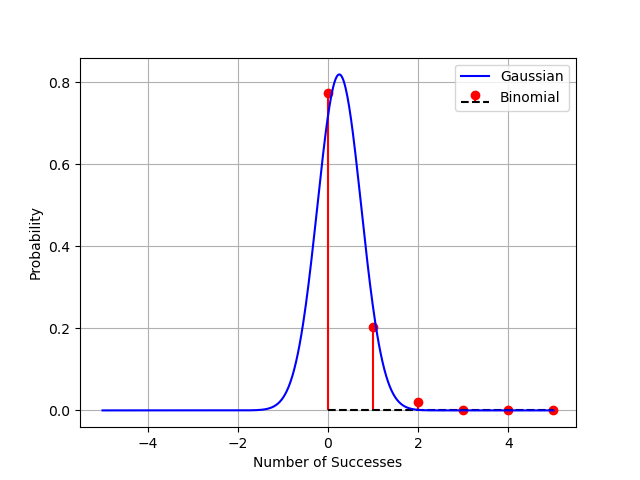
\includegraphics[width=\columnwidth]{./figs/bg.png}
\caption{Binomial vs guassian}
\label{fig:BvG_py}
\end{figure}
\end{document}
